\subsection{Presentation}

L'objectif de notre projet d'étude et de développement est de produire une bibliothèque d'extraction et d'analyse d'images à partir d'un flux vidéo. Cette bibliothèque sera utilisée pour des applications de vision par ordinateur.\\

L'extraction d'images consiste à récupérer un espace de dessin dans la vidéo. cet espace de dessin peut être une feuille blanche, entourée par une planche de tags. Au début du projet, une bibliothèque d'extraction (\texttt{ARToolkit}) nous a été fournie. Nous devions donc nous concentrer sur les analyses des images obtenues.\\

Les analyses demandées par ce projet sont de deux types : 
\begin{itemize}
\item Une analyse rapide, sur une image de faible qualité. Le but de cette analyse est de retrouver des formes simples (voir les templates ci-dessous) dans le dessin.
\item Une analyse sur des images de haute qualité. Cette analyse a pour but de détecter les nouveautés dans le dessin.\\
\end{itemize}
Des applications utilisant la bibliothèque sont également à développer, notamment une application de détection de nouveautés dans un dessin, et une application de reconnaissance de formes simples.

\begin{center}
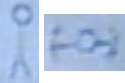
\includegraphics[scale=1]{images/templates.png}
\captionof{figure}{\\Exemples de templates}
\end{center}

% Extraction : développer, dire qu'elle est fournie
% Analyse : Deux types : rapide, HD
% Analyse d'un dessin.

\subsection{Contexte}
contexte et existant sift surf etc...
Detection nouveauté article